\documentclass[spanish]{assignment}

% Title page
\title{Neurocomputación}
\subtitle{Práctica 1 - Introducción a las Redes Neuronales Artificiales}
\author{Enrique Cabrerizo Fernández\\ Guillermo Ruiz Álvarez}
\date{\today}
\university{Universidad Autónoma de Madrid}

\begin{document}
	\makepre
	\section{Neuronas de McCulloch-Pitts}
	En esta sección se detallará el diseño de una red con neuronas de \textbf{McCulloch-Pitts} que resuelven el problema propuesto en el enunciado de la práctica. En la figura \ref{fig:nnet} se puede observar la estructura de la red, en la que:
	\begin{itemize}
		\item Las neuronas $X_1, X_2$ y $X_3$ son los nodos de entrada, $Y_1$ e $Y_2$ son los nodos de salida, $Z_1, Z_2, Z_3$ son los nodos de la primera capa oculta, y $Z_4, \hdots, Z_9$ son los nodos de la segunda capa oculta. 
		\item En cada nodo de la red, $\theta$ indica el valor del umbral. 
		\item Los valores de las conexiones entre neuronas representan el peso en cada caso. En esta red se ha escogido el valor $1$ para todas las conexiones excitadoras y $-2$ para las conexiones inhibidoras.
	\end{itemize}
	\fimg{NNet.png}{width=25em}{Red de neuronas McCulloch-Pitts}{nnet}
	
	\subsection{Descripción del diseño de la red}
	En el problema propuesto se especifica que la salida de la red en el instante $t$ ha de depender de la orientación del estímulo en $t-1$ con respecto al estímulo en $t-2$. Sin embargo, en el diseño realizado, la salida en el instante $t$ depende de la orientación del estímulo en $t-2$ con respecto al estímulo en $t-3$.
	
	Esto se debe a que, dado que se requiere un paso de tiempo para que una señal pase a través de una conexión, se necesitan al menos dos capas ocultas: una para almacenar el primer estímulo entrante y otra para realizar la comparación entre el estímulo almacenado y el consecutivo. 
	
	\subsubsection{Primera capa oculta}
	Pasado el primer instante de tiempo, los valores de la entrada de la red se propagan a la primera capa oculta. Para ello, todas las conexiones entre la capa de entrada y la primera capa oculta son excitadoras (con valor $1$) y los valores de umbral de los nodos $Z_1, Z_2, Z_3$ son en todos los casos $\theta = 1$.
	
	\subsubsection{Segunda capa oculta}
	En el segundo instante de tiempo, a cada nodo de la segunda capa oculta llegan los valores de dos nodos: uno de la entrada en el instante actual y uno de la entrada en el instante anterior (que está almacenado en la primera capa oculta). De esta forma, se pueden comparar los nodos de dos entradas consecutivas.
	
	Los nodos $Z_4, Z_5, Z_6$ comprueban si se ha producido un desplazamiento hacia abajo, y los nodos $Z_7, Z_8, Z_9$ comprueban si se ha producido desplazamiento hacia arriba.	Los valores llegan con peso $1$ a las neuronas de la segunda capa oculta, que tienen todas umbral $\theta=2$, es decir, cada nodo de la segunda capa oculta se activa sólo si los valores que llegan son ambos $1$.
	
	Si $Z_4, Z_5$ o $Z_6$ tienen un valor $1$, activarán la neurona de salida $Y_2$ y desactivarán la neurona de salida $Y_1$. Si $Z_7, Z_8$ o $Z_9$ tienen un valor $1$, activarán la neurona de salida $Y_1$ y desactivarán la neurona de salida $Y_2$. De esta manera, al tener un peso de $-2$ para la desactivación, se controlan las entradas inválidas haciendo que la salida para cualquier entrada invalida sea $(0\ 0)$, ya que se produce la desactivación de ambas neuronas si se detectan subidas y bajadas simultaneamente.
	
	Por otro lado, ya que las seis neuronas de la segunda capa oculta nunca comparan nodos que estén a la misma altura (es decir, $X_i$ con $Z_i$, para $i=1,2,3$), si se tienen dos entradas consecutivas iguales, la segunda capa oculta tendrá todos sus nodos a $0$, y por tanto la salida será $(0\ 0)$.

	\newpage
	\paragraph{Ejemplo:}
	A continuación se muestra un ejemplo en el que se detalla el comportamiento de la red en cada iteración temporal hasta producir la salida. Sean los siguientes estímulos:
	\begin{center}
		\begin{tabular}{c|c|c|}
			& $t$ & $t+1$ \\
			\hline
			$X_1$ & $0$ & $1$   \\
			$X_2$ & $0$ & $0$   \\
			$X_3$ & $1$ & $0$  
		\end{tabular}
	\end{center}
	
	En la figura \ref{fig:nnetex1} se puede observar como evoluciona la red ante los estímulos descritos en la tabla anterior.
	
	\fimg{NNetEx1.png}{width=25em}{Evolución de la red de neuronas McCulloch-Pitts}{nnetex1}
	
	\begin{itemize}
	\item En el instante $t$ entra el primer estímulo.
	\item En el instante $t+1$ entra el segundo estímulo de forma que en la capa de entrada y en la primera capa oculta se tienen ambos almacenados.
	\item En el instante $t+2$ se realizan todas las comprobaciones de bajada en los tres primeros nodos de la segunda capa oculta y todas las comprobaciones de subida en los tres últimos nodos de la misma capa. Se puede observar que el primer nodo detecta que se ha producido una bajada del tercer bit de la primera entrada al primer bit de la segunda, porque dicho nodo tiene umbral $\theta=2$ y ambos nodos llegan activos con peso $1$.
	
	\item En el instante $t+3$ se realiza una operacion \texttt{OR} de los tres primeros nodos de la segunda capa oculta, activándose el segundo nodo de la salida.
	\end{itemize} 
	
	\subsection{Codificación de la red neuronal}
	El problema se ha resuelto utilizando \textsc{Octave}, por tanto, en lo que sigue se utilizará el lenguaje matricial para describir la codificación. La red neuronal se ha representado utilizando un grafo mediante una matriz de adyacencia con pesos. De esta forma, la matriz $A = (a_{ij})_{N\times N}$, donde $N=14$ es el número de nodos de la red, cumple que la entrada $a_{ij}$ será
	\begin{equation*}
		a_{ij} = 
		\left\{
		\begin{array}{l l}
		0 & \text{Los nodos } i,j \text{ no están conectados}\\
		1 & \text{Los nodos } i,j \text{ tienen una conexión excitadora}\\
		-2 & \text{Los nodos } i,j \text{ tienen una conexión inhibidora}
		\end{array}
		\right.
	\end{equation*}
	
	De esta forma, si $v_t$ es un vector de tamaño $N$ con el estado de la red en el instante $t$, y $\theta$ es un vector de tamaño $N$ donde cada entrada representa el umbral de cada nodo, el estado en $t+1$ se obtiene como:
	$$v_{t+1} = \left(v_t^T\cdot A\right) \ge \theta$$
	
	Donde $v_t^T$ representa el vector $v_t$ traspuesto y $\ge$ es un operador matricial que compara entrada a entrada dos vectores devolviendo $1$ si la primera entrada es mayor o igual que la segunda y $0$ en caso contrario.
	
	\newpage
	\section{Perceptrón y Adaline}
	En esta sección se describe el diseño dos tipos de redes neuronales artificales: el Perceptrón y el Adaline. El diseño de ambas redes es similar, cambiando en cada caso la regla de aprendizaje. Tanto para el Perceptrón como para el Adaline se ha utilizado un esquema con varias neuronas de salida, es decir, tendremos tantas neuronas de salida como clases posibles.
	
	\subsection{Diseño y estructura}
	Ambas redes se han diseñado utilizando \textsc{Octave}, por tanto, en lo que sigue se utilizará el lenguaje matricial para describir la codificación.
	Llamaremos $n$ al número de parámetros que se utilizan para la clasificación, y $m$ al número de clases posibles. Tenemos: 
	\begin{itemize}
		\item $x$: un vector fila de tamaño $n$, representando los parámetros que se utilizan para la clasificación.
		\item $w$: una matriz $m\times n$, donde cada fila es el conjunto de pesos utilizado para clasificar cada clase.
		\item $b$: un vector columna de tamaño $m$, donde cada elemento representa el sesgo utilizado para clasificar cada clase.
		\item $y$: un vector columna de tamaño $m$, representando el resultado de la clasificación para cada clase.
	\end{itemize}
	De este modo, si llamamos:
	$$y_{in} = b + w\cdot x^T$$
	Entonces, la salida de la red vendrá dada por
	$$y = F\left(y_{in}\right)$$
	donde $F$ es una función matricial que aplica la función $f$ de transferencia a cada elemento del vector $y_{in}$ obtenido.
	
	
	\newpage
	\subsection{Experimentos realizados}
	En este apartado se discutirán los resultados obtenidos para cada problema resuelto.
	\subsubsection{Primer problema real}
	Se ha realizado un programa que lee los datos del problema y realiza una partición aleatoria de los mismos utilizando un $70\%$ para el conjunto de entrenamiento y un $30\%$ para el conjunto de test. Finalmente, entrena la red y además de ofrecer los resultados especificados en el enunciado, se escribe un fichero de salida con tres columnas, donde cada una de ellas representa:
	\begin{enumerate}
		\item Número de época.
		\item Error cometido.
		\item Error cuadrático medio.
	\end{enumerate}
	
	Se han probado varios valores para la tasa $\alpha$ de aprendizaje y para el umbral $\theta$ en el caso del Perceptrón. 
	A continuación se exponen los resultados para 50 épocas:
	
	\paragraph{Datos para el Perceptrón:} Se expone el valor del error en función de los valores de $\alpha$ y $\theta$.
	\begin{center}
		\begin{tabular}{|c|c|c|}
			\hline
			\textbf{Valor de $\alpha$} & \textbf{Valor de $\theta$} & \textbf{Error}\\
			\hline
			$0.1$ & $0$ & $3.27\%$\\
			$0.5$ & $0$ & $5.73\%$\\
			$1$ & $0$ &  $5.11\%$\\
			\hhline{|=|=|=|}
			$0.1$ & $0.2$ & $4.91\%$\\
			$0.5$ & $0.2$ & $4.10\%$\\
			$1$ & $0.2$ &  $4.90\%$\\
			\hline
		\end{tabular}
	\end{center}
	\paragraph{Datos para el Adaline:} Se expone el valor del error cuadrático medio en función del valor de $\alpha$.
	\begin{center}
		\begin{tabular}{|c|c|c|}
			\hline
			\textbf{Valor de $\alpha$} & \textbf{Error cuadrático medio}\\
			\hline
			$0.01$  & $0.282$\\
			$0.05$ & $0.318$\\
			$0.1$  & $0.357$\\
			\hline
		\end{tabular}
	\end{center}
	
	En ningún caso las redes convergen completamente, incluso para un valor más alto de épocas. Por tanto, aunque la aproximación sea muy buena, al no tener convergencia se puede concluir que el problema no es linealmente separable.
	
	\begin{center}
	\begin{figure}
		\makebox[\textwidth][c]{
			\begin{subfigure}[h]{0.55\textwidth}
				\centering
				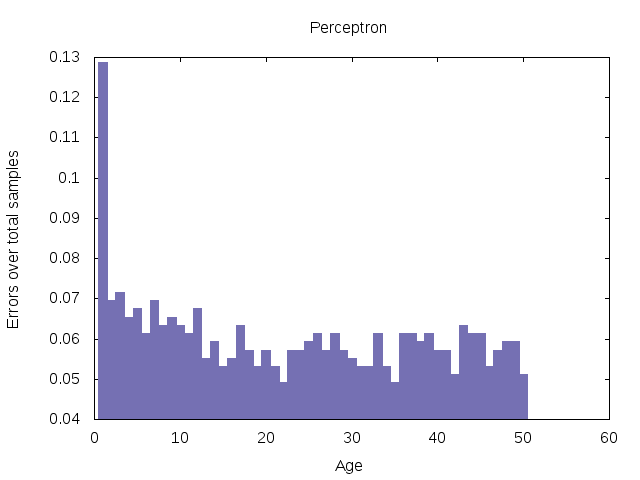
\includegraphics[width=\textwidth]{p1_perc.png}
				\caption{Error en el Perceptrón para $\alpha =$ 0.1, $\theta =$ 0}
			\end{subfigure}		
			\begin{subfigure}[h]{0.55\textwidth}
				\centering
				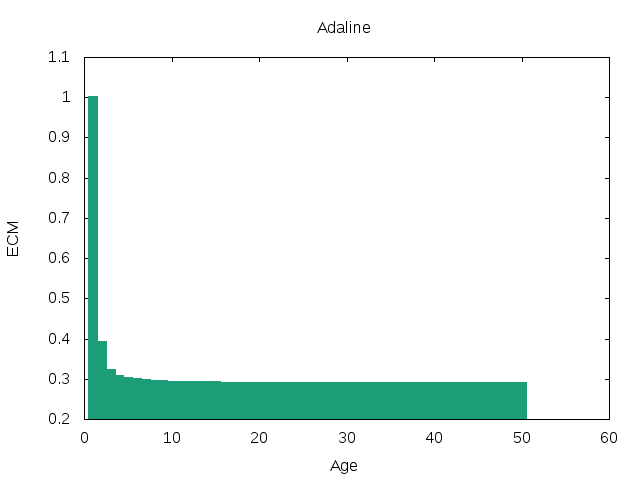
\includegraphics[width=\textwidth]{p1_ada.png}
				\caption{ECM en el Adaline para $\alpha =$ 0.01}
			\end{subfigure}%
		}
		\caption{Evolución de errores para el Perceptrón y Adaline.}	
		\label{fig:p1}
	\end{figure}
	\end{center}
	En la figura \ref{fig:p1} se ha representado, por un lado, como evoluciona el error en el Perceptrón en cada época de entrenamiento, observándose que el valor de $\alpha$ utilizado no produce oscilaciones muy grandes en el error. Por otro lado, se ha representado la evolución del error cuadrático medio en el Adaline, observándose que, efectivamente, la regla delta de aprendizaje lo minimiza.
	
	\subsubsection{Problemas con puertas lógicas}
	Para resolver los problemas dados por los datos de las bases \textsc{nand}, \textsc{nor} y \textsc{xor}, se ha utilizado el conjunto completo tanto para la fase de entrenamiento como para la de test, un valor de $\alpha = 0.1$ para ambas redes y un valor de $\theta = 0$ para el Perceptrón.
	
	En el caso de \textsc{nand} y \textsc{nor}, las redes obtienen un $100\%$ de acierto sobre el conjunto sobre el que han sido entrenadas, ya que estos problemas son linealmente separables. Sin embargo, ninguna de las redes es capaz de resolver el caso del \textsc{xor}, obteniéndose un $0\%$ de acierto, ya que este problema es claramente no separable. 
	
	\textbf{Nota: } En el caso del \textsc{xor}, aunque el conjunto de entrenamiento y de test sea el mismo, los porcentajes de acierto observados pueden cambiar. Esto se debe a que después del aprendizaje se tienen las muestras separadas linealmente, y cuando se realiza el test, las redes devuelven una clase porque no es aceptable no realizar una predicción. 
	
	\subsubsection{Segundo problema real}
	Se han aplicado el Percpetrón con parámetros $\alpha = 0.1$ y $\theta = 0$ y el Adaline con $\alpha = 0.01$ a los datos del segundo problema real. 
	
	\newpage
	En el caso del Perceptrón, se ha obtenido alrededor de un $70\%$ de acierto para el conjunto de entrenamiento y un $60\%$ para el conjunto de test. En el caso del Adaline, se ha obtenido alrededor de un $75\%$ de acierto tanto para el conjunto de entrenamiento como para el conjunto de test.

	En la figura \ref{fig:p2} se puede observar que el error en el caso del Perceptrón oscila alrededor del $30\%$ y, 
	en el caso del Adaline, el error cuadrático medio parece tener una cota inferior alrededor de $1.3$. Observando estos resultados se puede deducir que el problema no es linealmente separable.
	\begin{center}
		\begin{figure}
			\makebox[\textwidth][c]{
				\begin{subfigure}[h]{0.55\textwidth}
					\centering
					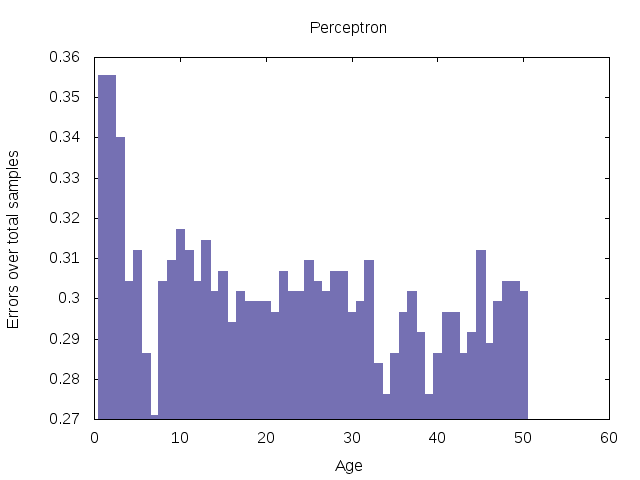
\includegraphics[width=\textwidth]{p2_perc.png}
					\caption{Error en el Perceptrón para $\alpha =$ 0.1, $\theta =$ 0}
				\end{subfigure}		
				\begin{subfigure}[h]{0.55\textwidth}
					\centering
					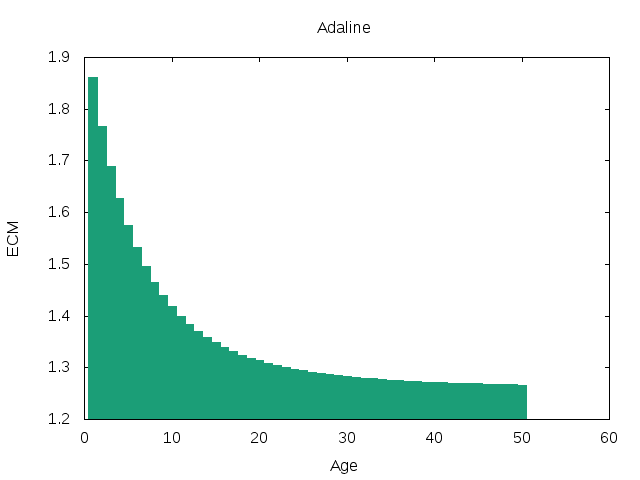
\includegraphics[width=\textwidth]{p2_ada.png}
					\caption{ECM en el Adaline para $\alpha =$ 0.01}
				\end{subfigure}%
			}
			\caption{Evolución de errores para el Perceptrón y Adaline.}	
			\label{fig:p2}
		\end{figure}
	\end{center}
	
	\subsubsection{Combinaciones no lineales.}
	Se han repetido los experimentos con los problemas \textsc{nand}, \textsc{nor} y \textsc{xor} y el segundo problema real añadiendo a los datos combinaciones no lineales de los mismos. Esto es, dado un conjunto de atributos y su respectiva clase, se han combinado productos por escalares y potencias de dichos atributos y se les ha asignado la misma clase. Por ejemplo, en el caso del segundo problema real, se han añadido atributos nuevos a partir del cuadrado de los atributos antiguo y se ha asignado la clase correspondiente en cada caso.
	
	En ningún caso las predicciones mejoran, de hecho, en todos los casos acaban empeorando, ya que estamos añadiendo datos no lineales. Es más, al añadir combinaciones no lineales de los atributos, estamos convirtiendo los problemas que eran linealmente separables en no linealmente separables. 
\end{document}